The case layer is the component that will house the physical components of the Traffic Pi system. This layer is comprised of four subsystems: a mounting plate, cooling, ventilation, and an interface. Each subsystem is responsible in some part for maintaining and protecting the physical components of the Traffic Pi system.

\subsection{Mounting Plate}
The mounting plate is detachable component of the case that can be attached to most camera tripods sold on the market. This subsystem is a part of the Traffic Pi system as a whole to facilitate the attaching of the system of a common item such as a tripod.

\begin{figure}[h!]
	\centering
 	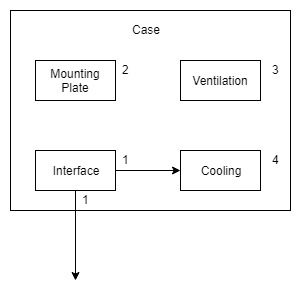
\includegraphics[width=0.60\textwidth]{images/case_layer}
 \caption{Case Layer Subsystem 2: Mounting Plate}
\end{figure}

\subsubsection{Assumptions}
It is assumed that the designed mounting plate included on the case for the Traffic Pi is suitable for mounting on most tripods on sold on the market.

\subsubsection{Responsibilities}
It is the responsibility of the mounting plate to provide the user of the Traffic Pi an easy to use location on the Traffic Pi such that a user may mount it to a standard camera tripod with ease.

\subsubsection{Subsystem Interfaces}
The interface for this subsystem is of a physical nature. The only input being the screw that is a detachable part of the mounting plate.

\begin {table}[H]
\caption {Mounting Plate interfaces} 
\begin{center}
    \begin{tabular}{ | p{1cm} | p{6cm} | p{3cm} | p{3cm} |}
    \hline
    ID & Description & Inputs & Outputs \\ \hline
    01 & Steel Screw 3/8 Inch & \pbox{3cm}{Steel Screw} & \pbox{3cm}{N/A}  \\ \hline
    \end{tabular}
\end{center}
\end{table}

\subsection{Cooling}
The cooling subsystem in the case layer is a component meant to keep the system within safe operating temperatures. This component draws power from the Raspberry Pi and operates whenever the Traffic Pi system is in use. 

\begin{figure}[h!]
	\centering
 	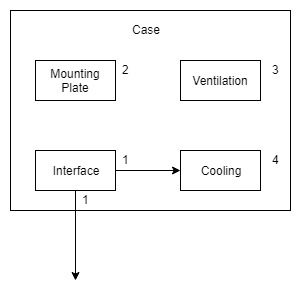
\includegraphics[width=0.60\textwidth]{images/case_layer}
 \caption{Case Layer Subsystem 4: Cooling}
\end{figure}

\subsubsection{Assumptions}
It is assumed that the cooling component of the case is able to draw sufficient power from the Raspberry Pi to operate efficiently. Further it is assumed that continued use of the cooling component will impact performance of the Traffic Pi system.

\subsubsection{Responsibilities}
It is the responsibility of the cooling subsystem to keep the Raspberry Pi, IR camera, and 3D camera in a temperature range that rated for these devices, -30 C to 80 C.

\subsubsection{Subsystem Interfaces}
The interface for this subsystem is of a physical nature. The only input being the screw that is a detachable part of the mounting plate.

\begin {table}[H]
\caption {Cooling Interfaces} 
\begin{center}
    \begin{tabular}{ | p{1cm} | p{6cm} | p{3cm} | p{3cm} |}
    \hline
    ID & Description & Inputs & Outputs \\ \hline
    04 & Power from the Raspberry Pi & \pbox{3cm}{Interface} & \pbox{3cm}{N/A}  \\ \hline
    \end{tabular}
\end{center}
\end{table}

\subsection{Ventilation}
The ventilation component of the case layer is intended to allow any heat generated by use of the Traffic Pi system to dissipate in a controlled manner. The Raspberry Pi in particular will generate heat upon use of the system and although a cooling component is available, this ventilation subsystem will allow further dissipation of heat.

\begin{figure}[h!]
	\centering
 	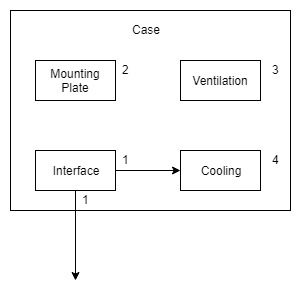
\includegraphics[width=0.60\textwidth]{images/case_layer}
 \caption{Case Layer Subsystem 3: Ventilation}
\end{figure}

\subsubsection{Assumptions}
It is assumed that this ventilation subsystem in conjunction with the cooling subsystem is sufficient enough to keep the system within safe operating temperatures.

\subsubsection{Responsibilities}
It is the responsibility of the ventilation subsystem to allow heat generated from the Raspberry Pi, IR camera, and 3D camera to safely dissipate away from the system.

\subsubsection{Subsystem Interfaces}
This component does not interact with any other subsystem.

\subsection{Interface}
The interface subsystem in the case layer is a component meant to provide power to the cooling subsystem which has been directed from the Traffic Pi. This interface is purely hardware in nature, a standard USB Type C cable. 

\begin{figure}[h!]
	\centering
 	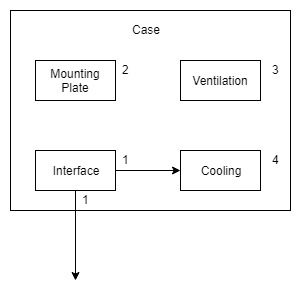
\includegraphics[width=0.60\textwidth]{images/case_layer}
 \caption{Case Layer Subsystem 1: Interface}
\end{figure}

\subsubsection{Assumptions}
It is assumed that the interface cable is able to transmit the necessary power requirements of the cooling subsystem from the Raspberry Pi.

\subsubsection{Responsibilities}
It is the responsibility of the interface to provide a conduit of power from the Raspberry Pi to the cooling subsystem.

\subsubsection{Subsystem Interfaces}
This subsystem interfaces with the Raspberry Pi and Cooling subsystems.

\begin {table}[H]
\caption {Interfaces} 
\begin{center}
    \begin{tabular}{ | p{1cm} | p{6cm} | p{3cm} | p{3cm} |}
    \hline
    ID & Description & Inputs & Outputs \\ \hline
    04 & USB Type C Cable & \pbox{3cm}{Power from Raspberry Pi} & \pbox{3cm}{Power to Cooling}  \\ \hline
    \end{tabular}
\end{center}
\end{table}